\documentclass{article}
\usepackage{amsmath}
\usepackage{float}
\usepackage{graphicx}
\usepackage{varwidth}
\usepackage{xcolor}
\usepackage{geometry}
\addtolength{\topmargin}{-.875in}
\addtolength{\textheight}{1.75in}

\newcommand{\block}[1]{%
  \begingroup
  \setlength{\fboxsep}{0pt}%
  \vrule width0pt height \blockdim
  \ooalign{%G
    \framebox[\blockdim]{\rule{0pt}{\blockdim}}\cr
    \hidewidth\raisebox{0.5\dimexpr\blockdim-\height}{\raisebox{\depth}{#1}}\hidewidth\cr
  }%
  \endgroup
}
\newcommand{\greenblock}[1]{%
  \begingroup
  \setlength{\fboxsep}{0pt}%
  \vrule width0pt height \blockdim
  \ooalign{%
    \colorbox{green!20}{\framebox[\blockdim]{\rule{0pt}{\blockdim}}}\cr
    \hidewidth\raisebox{0.5\dimexpr\blockdim-\height}{\raisebox{\depth}{#1}}\hidewidth\cr
  }%
  \endgroup
}
\newcommand{\joinblocks}{\unskip\kern-\fboxrule\ignorespaces}
\newenvironment{blocks}[1][1cm]
 {\begin{varwidth}{\textwidth}\setlength{\blockdim}{#1}\makeblocks}
 {\end{varwidth}}
\newcommand{\makeblocks}{%
  \begingroup\lccode`~=`&\lowercase{\endgroup\let~}\joinblocks
  \catcode`\&=\active
  \baselineskip=0pt
  \lineskiplimit=\maxdimen
  \lineskip=0pt
  \centering
}
\newlength{\blockdim}

\begin{document}

1. In the pyramids below, a number in a cell is a sum of the numbers in the two cells below. Fill in the missing numbers.


\begin{blocks}
  \block{20}\\
  \block{} & \block{} \\
  \block{} & \block{5} & \block{} \\
  \block{3} & \block{1} & \block {} & \block{}
\end{blocks}
\begin{blocks}
  \block{20}\\
  \block{} & \block{} \\
  \block{} & \block{5} & \block{} \\
  \block{3} & \block{} & \block {1} & \block{}
\end{blocks}
\begin{blocks}
  \block{51}\\
  \block{} & \block{} \\
  \block{15} & \block{} & \block{18} \\
  \block{} & \block{6} & \block{} & \block{}
\end{blocks}


\vspace{3mm}

2. In the pyramids below, fill in the missing numbers. Pay attention to the additional conditions.

\begin{blocks}
  \block{12}\\
  \block{} & \block{} \\
  \block{} & \greenblock{} & \block{} \\
  \block{} & \greenblock{} & \block {0} & \block{1}
\end{blocks}
\begin{blocks}
\greenblock{} + \greenblock{} = 4
\end{blocks}
\begin{blocks}
  \block{}\\
  \block{} & \block{} \\
  \greenblock{} & \block{} & \block{} \\
  \block{4} & \greenblock{} & \block {7} & \block{0}
\end{blocks}
\begin{blocks}
\greenblock{} + \greenblock{} = 6
\end{blocks}


\vspace{3mm}

3. In the diagrams below, the arrows of the same color stand for the same number. The following must hold: "value at arrow start" + "arrow value" = "value at arrow target". Fill in the missing numbers.

\begin{figure}[H]
  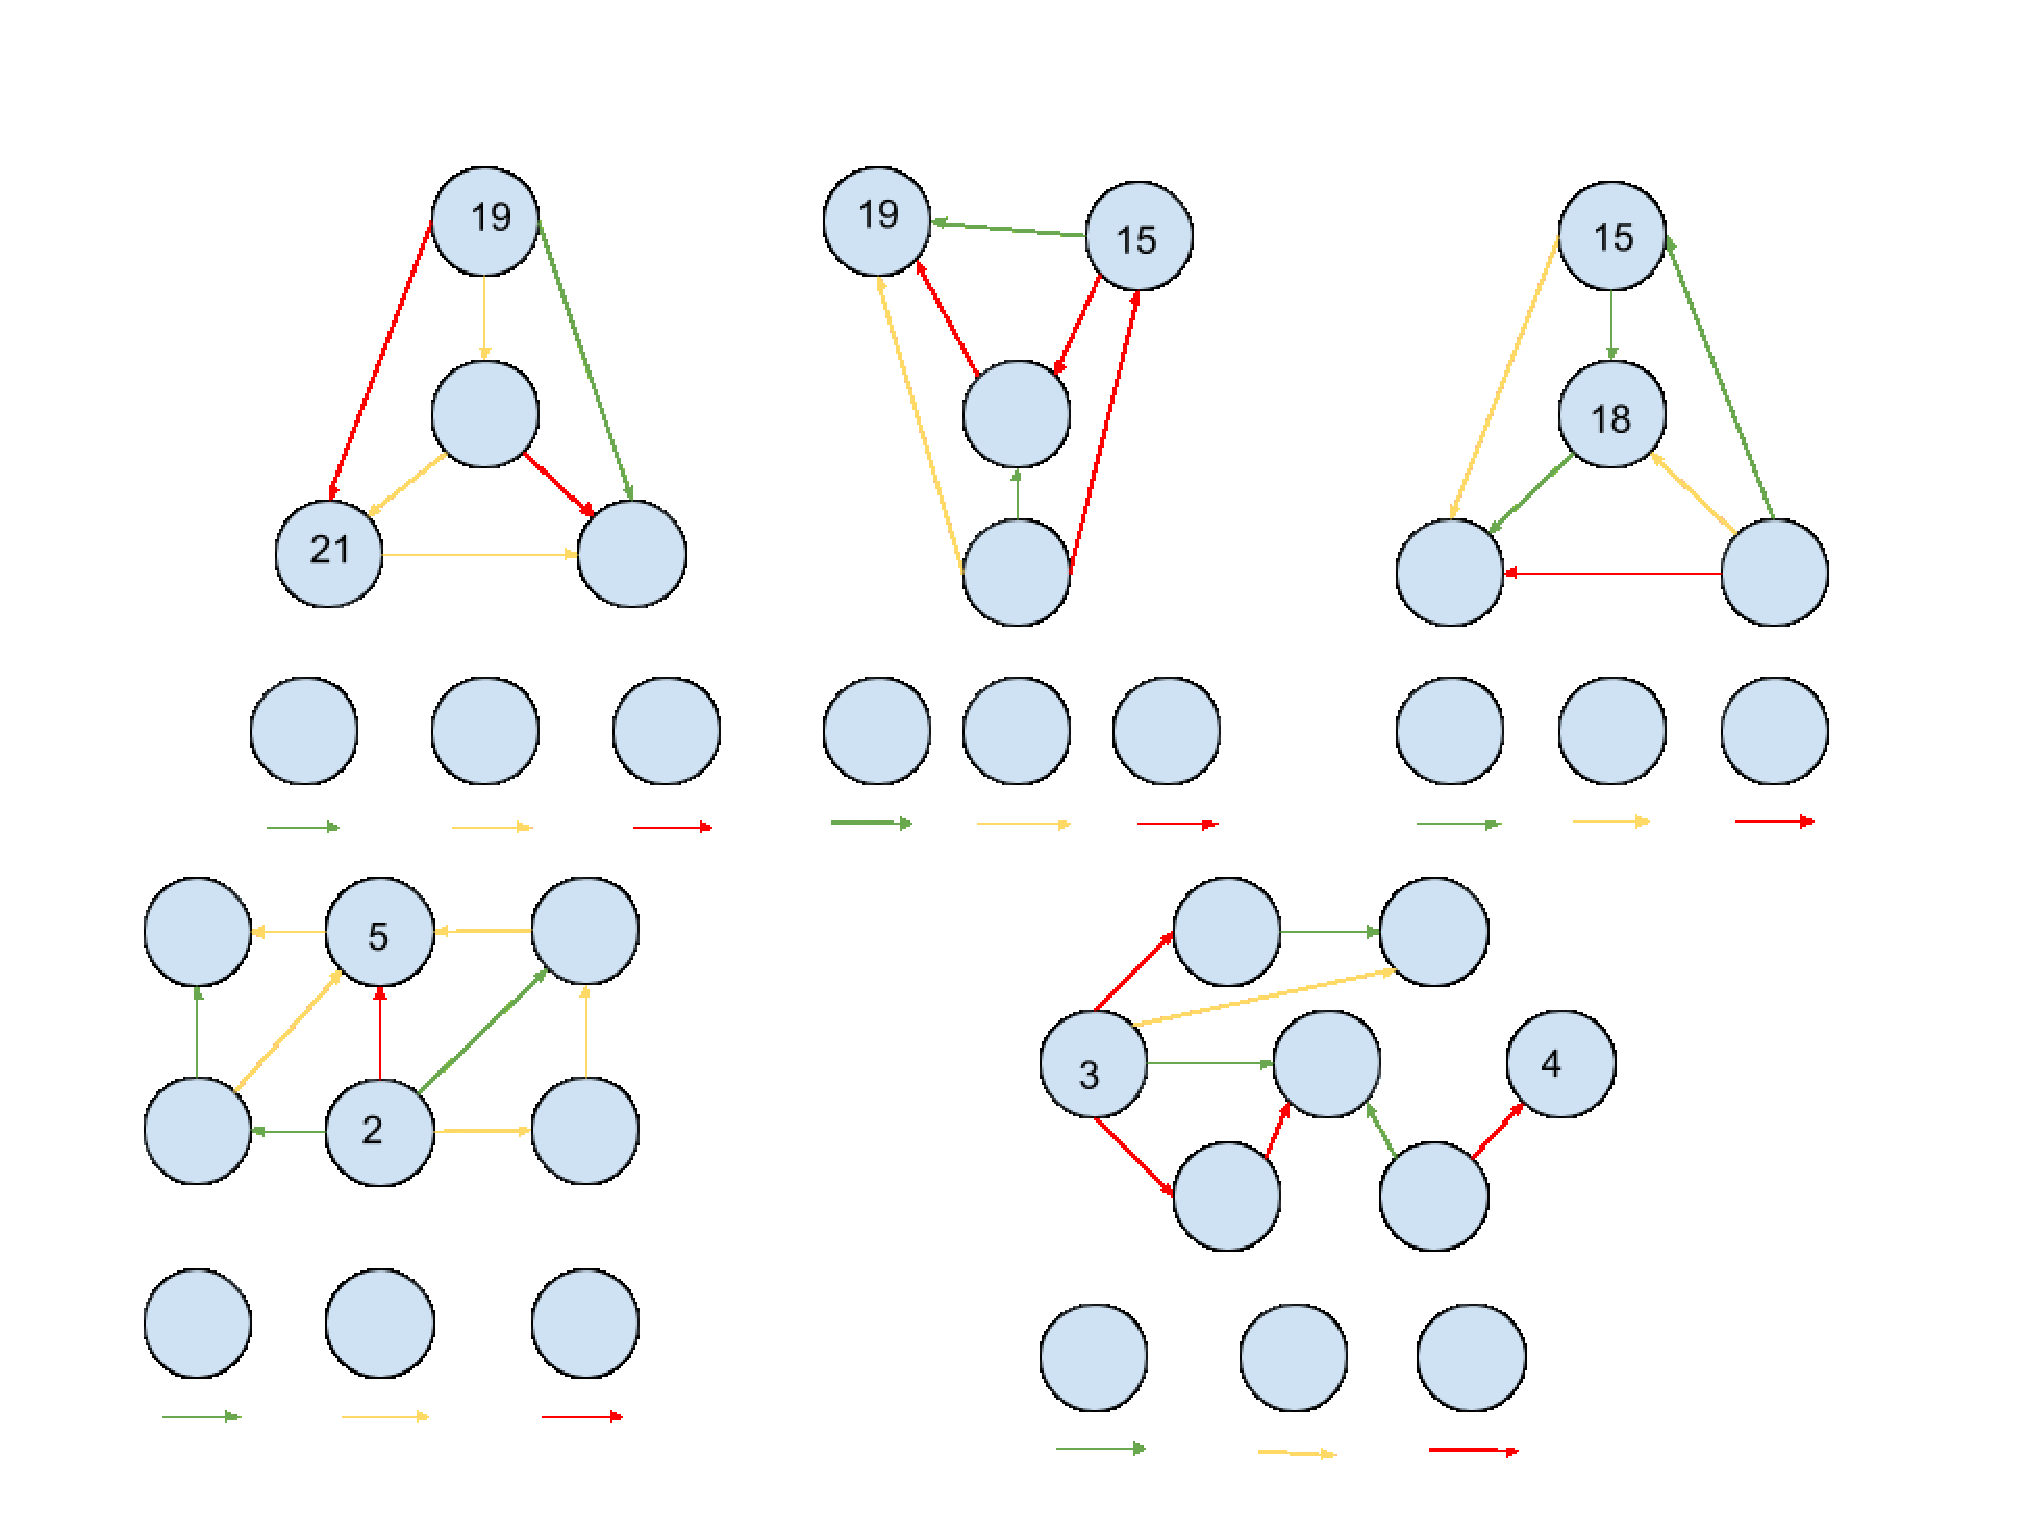
\includegraphics[width=0.8\textwidth]{pavuciny.eps}
\end{figure}


\vspace{3mm}

4. There are two bus lines connecting the stops A, B, C, D, E, F, G: C-A-F-G-E and A-E-D-B-G. Complete the picture with bus stop names.

\begin{figure}[H]
  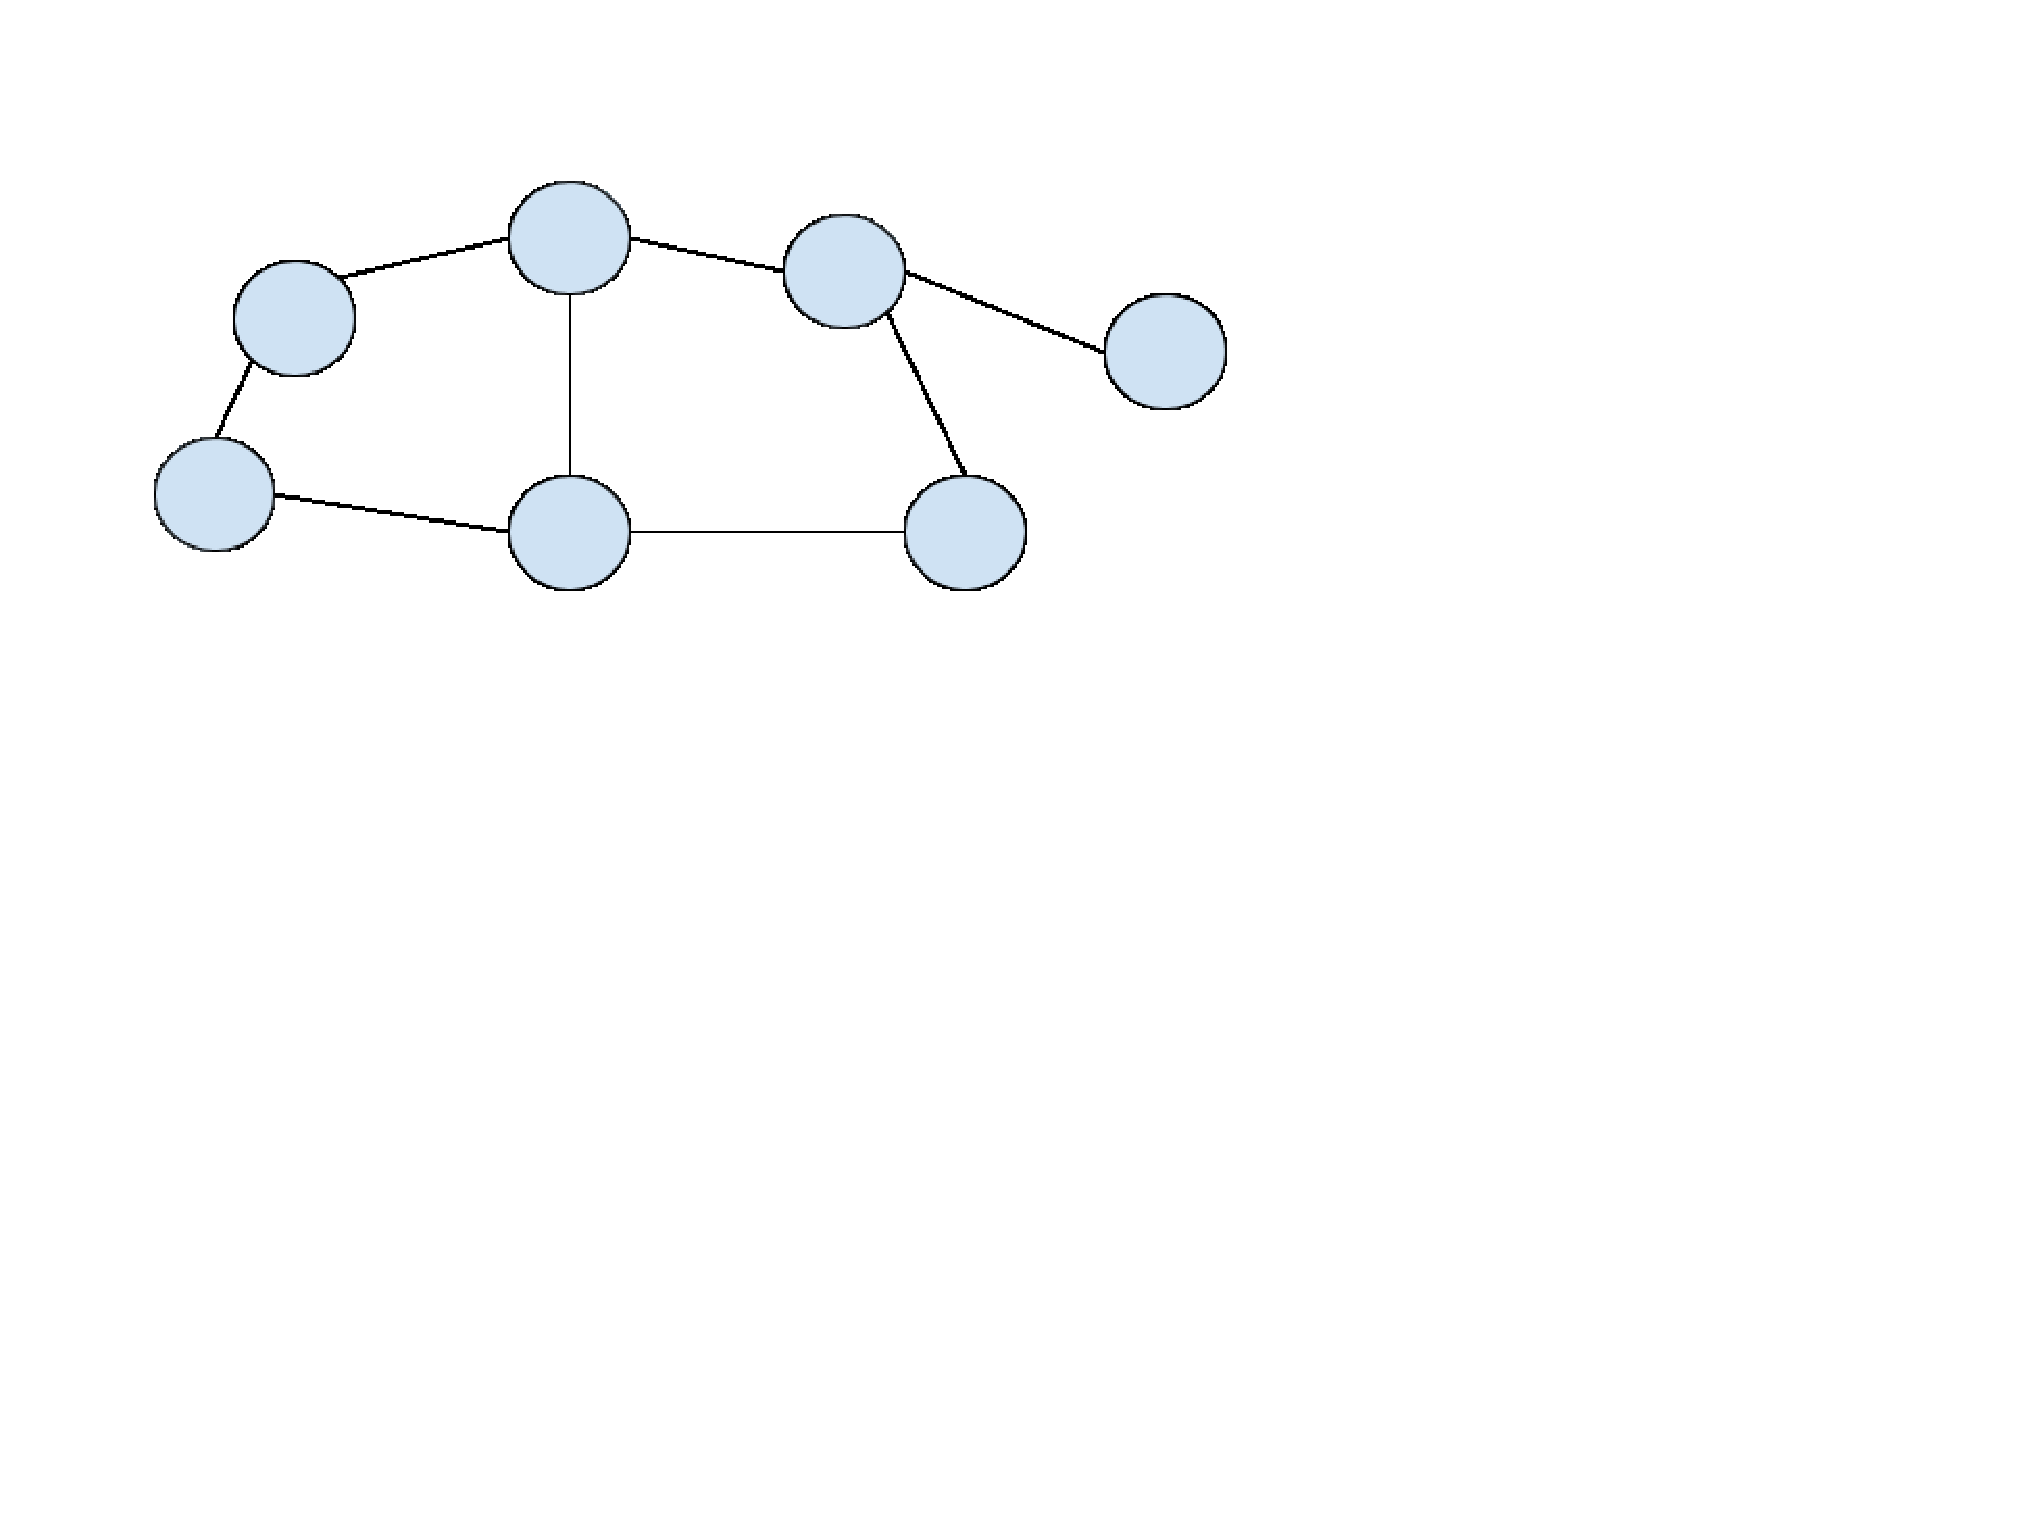
\includegraphics[width=0.8\textwidth]{buses.eps}
\end{figure}


\vspace{3mm}

5. Alice and Bob play the following game: One player picks a number from 1, 2, 3, .., 16, the other player is allowed to ask questions that the first player can answer with yes/no. Alice says she can always guess Bob's number with only 4 questions. Is that true?


\vspace{3mm}

6. Three siblings put together their money and bought a ball. Peter paid a half, Paul a quarter, and Mary the remaining \$2. How much did the ball cost?


\vspace{3mm}

7. There are 21 students in a class, 11 of them boys. 12 students play some instrument, 1/3 of them are boys. How many children don't play any instruments, how many of them are girls, how many are boys?
\end{document}
